\documentclass{article}
\usepackage{tikz}                                                                                                                                                  \usetikzlibrary{positioning}

\begin{document}
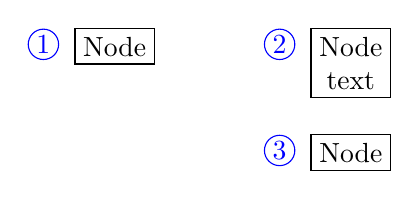
\begin{tikzpicture}[  
node distance = 4.5mm and 12mm,  % <---   
 block/.style = {draw, semithick, align=center, inner sep=3pt},
  circ/.style = {circle, draw, blue, inner sep=1pt,
                 node distance =2pt and 7pt}  % 2pt = 3pt (of block) - 1pt (of circle)}
                    ]
\node[block,below] (n1) {Node};                                                                                                                                          \node[circ,below left=of n1.north west] {1};

\node[block,below] (n2) at (3,0) {Node\\ text};                                                                                                                                          \node[circ,below left=of n2.north west] {2};

\node[block,below=of n2] (n3) {Node};                                                                                                                                          \node[circ,below left=of n3.north west] {3};
    \end{tikzpicture}
\end{document}